\section{Einstieg Berechnenbarkeit}
        
\subsection{Diagonalisierung}


    \textbf{Bijektion, Injektion, Schreibweise}
    \begin{mainbox}{}
        Seien $A$ und $B$ zwei Mengen.

        Wir sagen, dass 
        \begin{enumerate}[label=\roman*.]
            \item $\mathbf{|A| \leq |B|}$, falls eine injektive Funktion $f: A \to B$ existiert.
            \item $\mathbf{|A| = |B|}$, falls $|A| \leq |B|$ und $|B| \leq |A|$.
            \item $\mathbf{|A| < |B|}$, falls $|A| \leq |B|$ und keine injektive Abbildung von $B$ nach $A$ existiert.
        \end{enumerate}
    \end{mainbox}
    \textbf{Zur Erinnerung:}
    \begin{center}
        $f: A \to B$ injektiv $\iff $ $\forall x,y \in A, x\neq y. f(x) \neq f(y)$
    \end{center}



    \textbf{Abzählbarkeit}
    \begin{mainbox}{}
        Eine Menge $A$ heisst \textbf{abzählbar}, falls $A$ endlich ist oder $|A| = |\N|$.
    \end{mainbox}
    \begin{subbox}{Lemma 5.1}
    Sei $\Sigma$ ein beliebiges Alphabet. Dann ist $\Sigma^*$ abzählbar.
    \end{subbox}
    % \textbf{Beweisidee}

    % kanonische Ordnung gibt uns eine Bijektion zwischen $\N$ und $\Sigma^*$.

    \begin{mainbox}{Satz 5.1}
        Die Menge \textbf{KodTM} der Turingmaschinenkodierungen ist abzählbar.
    \end{mainbox}
    \textbf{Beweisidee}

    KodTM $\subseteq (\Sigma_{\text{bool}})^*$ und Lemma 5.1

    \begin{mainbox}{Lemma 5.2}
        $(\N\setminus\{0\}) \times (\N \setminus \{0\})$ ist abzählbar.
    \end{mainbox}
    \textbf{Beweisidee}

    Unendliche 2-dimensionale Tabelle, so dass an der $i$-ten Zeile und $j$-ten Spalte, sich das Element $(i,j) \in (\N\setminus\{0\}) \times (\N \setminus \{0\})$ befindet.

    Formal definiert man dabei die lineare Ordnung 
    $$(a,b) < (c,d) \iff a+b < c+d \text{ oder }(a+b = c+d \text{ und } b <d)$$

    \begin{figure}[htp]
        \includegraphics[width=0.7\textwidth]{Images/Abzählen.png}
        \caption{Abbildung 5.3 im Buch}
    \end{figure}

    Die $i$-te Diagonale hat $i$ Elemente. Ein beliebiges Element $(a,b) \in (\N\setminus\{0\}) \times (\N \setminus \{0\})$ ist das $b$-te Element auf der $(a+b-1)$-ten Diagonale.
    
    Auf den ersten $a+b-2$ Diagonalen gibt es 
    $$\sum_{i = 1}^{a+b-2}i = \frac{(a+b-2)\cdot((a+b-2)+1)}{2} = \binom{a+b-1}{2}$$
    Elemente.

    Folglich ist 
    $$f((a,b)) = \binom{a+b-1}{2} + b$$
    eine Bijektion von $(\N\setminus\{0\}) \times (\N \setminus \{0\})$ nach $\N\setminus\{0\}$.



    \textbf{Überabzählbarkeit}

    \begin{mainbox}{Satz 5.3}
        $[0,1]$ ist nicht abzählbar.
    \end{mainbox}
    \textbf{Beweisidee}
    
    Klassisches Diagonalisierungsargument. Aufpassen auf $0$ und $9$. I.e. $1 = 0.\overline{99}$.

    \begin{figure}[htp]
        \includegraphics[width=0.7\textwidth]{Images/Diagonalisierung.png}
    \end{figure}

    \begin{mainbox}{Satz 5.4}
        $\mathcal{P}((\Sigma_{\text{bool}})^*)$ ist nicht abzählbar.
    \end{mainbox}
    \textbf{Beweis: }

        Wir definieren eine injektive Funktion von $f: [0, 1] \to \mathcal{P}((\Sigma_{bool})^*)$ und beweisen so $|\mathcal{P}((\Sigma_{bool})^*)| \geq |[0, 1]|$.
    
        Sei $a \in [0, 1]$ beliebig. Wir können $a$ wie folgt binär darstellen:
        $$\text{Nummer}(a) = 0.a_1a_2a_3a_4... \text{ mit } a = \sum_{i = 1}^{\infty} a_i\cdot 2^{-i}.$$ 
        
        Hier ist zu beachten, dass wir für eine Zahl $a$ immer die lexikographisch letzte Darstellung wählen.
    
    Dies tun wir, weil eine reelle Zahl 2 verschiedene Binärdarstellungen haben kann. Beispiel: $\frac{1}{2} = 0.1\overline{0} = 0.0\overline{1}$.
        
        Für jedes $a$ definieren wir:
        $$f(a) = \{a_1, a_2a_3, a_4a_5a_6, ..., a_{\binom{n}{2}+1}a_{\binom{n}{2}+2}...a_{\binom{n+1}{2}} , ...\}$$
    
        Da $f(a) \subseteq (\Sigma_{bool})^*$ gilt $f(a) \in \mathcal{P}((\Sigma_{bool})^*)$.
    
        Wir haben für alle $n \in \N \setminus\{0\}$, dass $f(a)$ \textbf{genau} ein Wort dieser Länge enthält. Nun können wir daraus folgendes schliessen:
    
        Weil die Binärdarstellung zweier unterschiedlichen reellen Zahlen an mindestens einer Stelle unterschiedlich ist, gilt $b \neq c \implies f(b) \neq f(c), \forall b,c \in [0, 1]$. 
    
        Folglich ist $f$ injektiv und wir haben $|\mathcal{P}((\Sigma_{bool})^*)| \geq |[0, 1]|$.
    
        Da $[0,1]$ nicht abzählbar ist, folgt daraus:
    
        $\mathcal{P}((\Sigma_{bool})^*)$ ist nicht abzählbar.
        
        \hspace*{0pt}\hfill$\blacksquare$



    \textbf{Diagonalsprache $L_{\text{diag}}$ }

    Zur Erinnerung:
    \begin{mainbox}{Rekursiv aufzählbare Sprachen}
        Eien Sprache $L \subseteq \Sigma^*$ heisst \textbf{rekursiv aufzählbar}, falls eine TM $M$ existiert, so dass $L = L(M)$.
        $$\mathbf{\mathcal{L}_{\textbf{RE}}} = \{L(M) \mid M \text{ ist eine TM}\}$$
        ist die \textbf{Klasse aller rekursiv aufzählbaren Sprachen}.
    \end{mainbox}
    Wir zeigen jetzt per Diagonalisierung, die Existenz einer Sprache die nicht rekursiv aufzählbar ist.


    Sei $w_1, w_2,...$ die kanonische Ordnung aller Wörter über $\Sigma_{\text{bool}}$ und sei $M_1, M_2, M_3,...$ die Folge aller Turingmaschinen.
    
    Wir definieren eine unendliche (bool'sche) Matrix $A = [d_{ij}]_{i,j = 1, 2, ...}$ mit 
    $$d_{ij} = 1 \iff M_i \text{ akzeptiert }w_j.$$

    Wir definieren
    $$L_{\text{diag}} = \{w \mid w = w_i \text{ und $M_i$ akzeptiert $w_i$ nicht für ein $i \in \N\setminus\{0\}$}\}$$


    \begin{mainbox}{Satz 5.5}
        $$L_{\text{diag}} \notin \L_{\text{RE}}$$
    \end{mainbox}

    \textbf{Beweis:}

    Wir haben 
    $$L_{\text{diag}} = \{w \mid w = w_i \text{ und $M_i$ akzeptiert $w_i$ nicht für ein $i \in \N\setminus\{0\}$}\}$$

    Widerspruchsbeweis:

    Sei $L_\text{diag} \in \L_{\text{RE}}$. Dann existiert eine TM $M$, so dass $L(M) = L_\text{diag}$. Da diese TM eine TM in der Nummerierung aller TM ist, existiert ein $i \in \N$, so dass $M_i = M$.

    Wir betrachten nun das Wort $w_i$ für diese $i \in \N$. Per Definition von $L_\text{diag}$, gilt:

    $$w_i \in L_\text{diag} \iff w_i \notin L(M_i)$$

    Da aber $L(M_i) = L_\text{diag}$, haben wir folgenden Widerspruch:
    $$w_i \in L_\text{diag} \iff w_i \notin L_\text{diag}$$

    Folglich gilt $L_\text{diag} \notin \L_\text{RE}$.
    
    \hspace*{0pt}\hfill$\blacksquare$


    
        \subsection{Klassifizierung verschiedener Sprachen}
        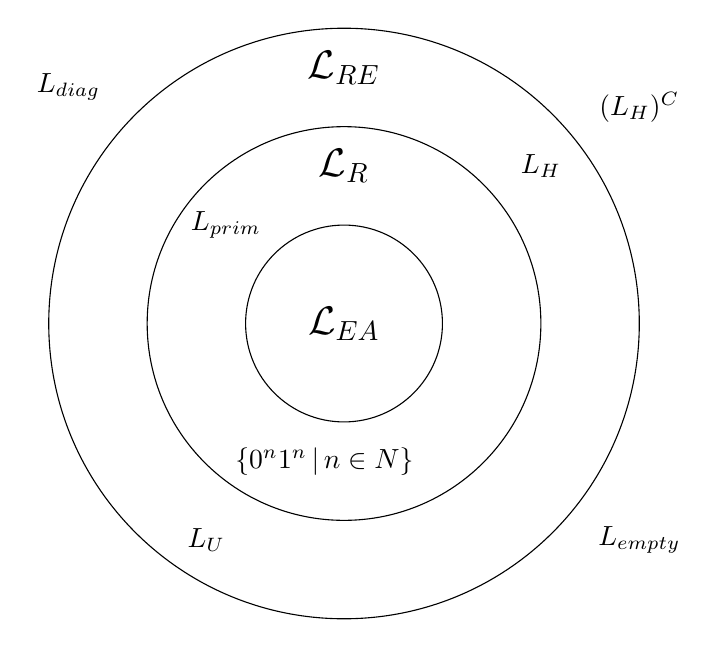
\begin{tikzpicture}
            \draw (0,0) circle (3.75);
            \draw (0,0) circle (2.5);
            \draw (0,0) circle (1.25);
            \node at (0, 3.25) {\Large$\mathcal{L}_{RE}$};
            \node at (0, 2.) {\Large$\mathcal{L}_R$};
            \node at (0, 0) {\Large$\mathcal{L}_{EA}$};
            
            % \node at (0, -0.25) {$\{|x|_a \mod 3 = 1\}$};
            \node at (-0.25, -1.75) {$\{0^n1^n \,|\, n\in \mathbb{N}\}$};
            \node at (-3.5, 3) {$L_\text{diag}$};
            \node at (2.5, 2) {$L_{H}$};
            \node at (-1.75, -2.75) {$L_{\text{U}}$};
            \node at (3.75, -2.75) {$L_\text{empty}$};
            \node at (3.75, 2.75) {$(L_{\text{H}})^C$};
            \node at (-1.5, 1.25) {$L_\text{prim}$};
            
        \end{tikzpicture}
    
    
    
        \myTitle{Begrifflichkeiten}

        Für eine Sprache $L$ gilt folgendes
        \begin{center}
            $L$ regulär $\iff $ $L \in \mathbf{\mathcal{L}_{\textbf{EA}}}$ $\iff$ $\exists$ EA $A$ mit $L(A) = L$\\
            $L$ rekursiv $\iff$ $L \in \mathbf{\mathcal{L}_{\textbf{R}}}$ $\iff$ $\exists$ Alg. A mit $L(A) = L$\\
            $L$ rekursiv aufzählbar $\iff$ $L \in \mathbf{\mathcal{L}_{\textbf{RE}}}$ $\iff$ $\exists$ TM $M$. $L(M) = L$
        \end{center}
        \begin{itemize}
            \item  ''Algorithmus'' $=$ TM, die immer hält.
            \item $L$ rekursiv $=$ $L$ entscheidbar
            \item $L$ rekursiv aufzählbar $=$ $L$ erkennbar
        \end{itemize}
       
